\section{Описание тестового стенда}

В результате работы в рамках ГПО в данном семестре был собран тестовый стенд, предназначенный для зеркалирования трафика с целью его последующего сбора.\par 

Тестовый стенд прозрачно включается в гигабитный канал связи Ethernet, после чего весь трафик, проходящий через стенд в любую сторону зеркалируется на выделенный сетевой интерфейс для его сбора отдельным модулем сбора и хранения трафика.\par 
 
Аппаратные требования, предъявляемые к тестовому стенду:
\begin{itemize}
	\item процессор Intel, поддерживающий архитектуру x86\_64;
	\item совместимая с процессором материнская плата, не менее чем с 4 слотами расширения PCI-Express;
	\item 3 сетевых карты PCI-Express производства Intel, с одним из следующих NIC: ixgbe (82598, 82599, 82557, X520, X540, X550), i40e (X710, XL710, X722);
	\item  сетевая карта PCI-Express для управления стендом;
	\item совместимый с материнской платой жесткий диск/твёрдотельный накопитель, объёмом не менее 20Gib;
	\item совместимая с материнской платой оперативная память, объёмом не менее 4Gib.
\end{itemize}

Программные требования, предъявляемые к тестовому стенду: операционная система Ubuntu 16.04 x86\_64.\par 

Итоговая аппаратная конфигурация тестового стенда:
\begin{itemize}
\item процессор Intel Core 2 6300 @ 1.86GHz;
\item материнская плата ASUS P5B;
\item сетевая карта PCI-Express Intel 82557/8/9/0/1 Ethernet Pro 100 (rev 05);
\item сетевая карта PCI-Express Intel 82557/8/9/0/1 Ethernet Pro 100 (rev 08);
\item сетевая карта PCI-Express Intel 82557/8/9/0/1 Ethernet Pro 100 (rev 08);
\item сетевая карта PCI-Express Realtek RTL8111/8168/8411 PCI Express Gigabit Ethernet Controller (rev 01);
\item жёсткий диск Seagate Barracuda, объёмом 250Gib;
\item оперативная память DDR2, объёмом 4Gib.
\end{itemize}

\clearpage

\begin{figure}[h!]
    \centering
    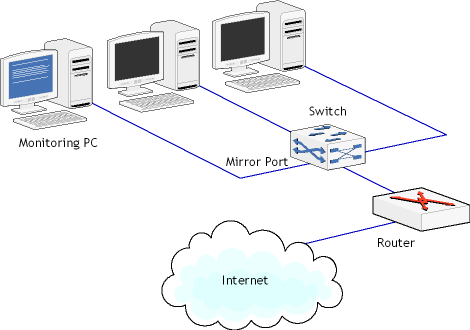
\includegraphics[width=0.7\textwidth]{8}
    \caption{Схема включения тестового стенда в сетевую инфраструктуру}
    \label{img:8}
\end{figure} 

Программная часть тестового стенда состоит из операционной системы Ubuntu 16.04 x86\_64 с установленным фреймворком DPDK, а также программы для зеркалирования трафика, написанной на языке C, с использованием библиотек DPDK.\par 

Перед началом работы сетевые интерфейсы стенда переводятся на использование DPDK-совместимых драйверов. После этого программа начинает зеркалировать весь трафик, проходящий между необходимыми сетевыми интерфейсами на зеркальный сетевой интерфейс. Для удалённого управления стендом используется выделенный сетевой интерфейс с запущенным SSH-сервером.\par 
